% Options for packages loaded elsewhere
\PassOptionsToPackage{unicode}{hyperref}
\PassOptionsToPackage{hyphens}{url}
\PassOptionsToPackage{dvipsnames,svgnames,x11names}{xcolor}
%
\documentclass[
  letterpaper,
  DIV=11,
  numbers=noendperiod]{scrartcl}

\usepackage{amsmath,amssymb}
\usepackage{iftex}
\ifPDFTeX
  \usepackage[T1]{fontenc}
  \usepackage[utf8]{inputenc}
  \usepackage{textcomp} % provide euro and other symbols
\else % if luatex or xetex
  \usepackage{unicode-math}
  \defaultfontfeatures{Scale=MatchLowercase}
  \defaultfontfeatures[\rmfamily]{Ligatures=TeX,Scale=1}
\fi
\usepackage{lmodern}
\ifPDFTeX\else  
    % xetex/luatex font selection
\fi
% Use upquote if available, for straight quotes in verbatim environments
\IfFileExists{upquote.sty}{\usepackage{upquote}}{}
\IfFileExists{microtype.sty}{% use microtype if available
  \usepackage[]{microtype}
  \UseMicrotypeSet[protrusion]{basicmath} % disable protrusion for tt fonts
}{}
\makeatletter
\@ifundefined{KOMAClassName}{% if non-KOMA class
  \IfFileExists{parskip.sty}{%
    \usepackage{parskip}
  }{% else
    \setlength{\parindent}{0pt}
    \setlength{\parskip}{6pt plus 2pt minus 1pt}}
}{% if KOMA class
  \KOMAoptions{parskip=half}}
\makeatother
\usepackage{xcolor}
\setlength{\emergencystretch}{3em} % prevent overfull lines
\setcounter{secnumdepth}{-\maxdimen} % remove section numbering
% Make \paragraph and \subparagraph free-standing
\ifx\paragraph\undefined\else
  \let\oldparagraph\paragraph
  \renewcommand{\paragraph}[1]{\oldparagraph{#1}\mbox{}}
\fi
\ifx\subparagraph\undefined\else
  \let\oldsubparagraph\subparagraph
  \renewcommand{\subparagraph}[1]{\oldsubparagraph{#1}\mbox{}}
\fi

\usepackage{color}
\usepackage{fancyvrb}
\newcommand{\VerbBar}{|}
\newcommand{\VERB}{\Verb[commandchars=\\\{\}]}
\DefineVerbatimEnvironment{Highlighting}{Verbatim}{commandchars=\\\{\}}
% Add ',fontsize=\small' for more characters per line
\usepackage{framed}
\definecolor{shadecolor}{RGB}{241,243,245}
\newenvironment{Shaded}{\begin{snugshade}}{\end{snugshade}}
\newcommand{\AlertTok}[1]{\textcolor[rgb]{0.68,0.00,0.00}{#1}}
\newcommand{\AnnotationTok}[1]{\textcolor[rgb]{0.37,0.37,0.37}{#1}}
\newcommand{\AttributeTok}[1]{\textcolor[rgb]{0.40,0.45,0.13}{#1}}
\newcommand{\BaseNTok}[1]{\textcolor[rgb]{0.68,0.00,0.00}{#1}}
\newcommand{\BuiltInTok}[1]{\textcolor[rgb]{0.00,0.23,0.31}{#1}}
\newcommand{\CharTok}[1]{\textcolor[rgb]{0.13,0.47,0.30}{#1}}
\newcommand{\CommentTok}[1]{\textcolor[rgb]{0.37,0.37,0.37}{#1}}
\newcommand{\CommentVarTok}[1]{\textcolor[rgb]{0.37,0.37,0.37}{\textit{#1}}}
\newcommand{\ConstantTok}[1]{\textcolor[rgb]{0.56,0.35,0.01}{#1}}
\newcommand{\ControlFlowTok}[1]{\textcolor[rgb]{0.00,0.23,0.31}{#1}}
\newcommand{\DataTypeTok}[1]{\textcolor[rgb]{0.68,0.00,0.00}{#1}}
\newcommand{\DecValTok}[1]{\textcolor[rgb]{0.68,0.00,0.00}{#1}}
\newcommand{\DocumentationTok}[1]{\textcolor[rgb]{0.37,0.37,0.37}{\textit{#1}}}
\newcommand{\ErrorTok}[1]{\textcolor[rgb]{0.68,0.00,0.00}{#1}}
\newcommand{\ExtensionTok}[1]{\textcolor[rgb]{0.00,0.23,0.31}{#1}}
\newcommand{\FloatTok}[1]{\textcolor[rgb]{0.68,0.00,0.00}{#1}}
\newcommand{\FunctionTok}[1]{\textcolor[rgb]{0.28,0.35,0.67}{#1}}
\newcommand{\ImportTok}[1]{\textcolor[rgb]{0.00,0.46,0.62}{#1}}
\newcommand{\InformationTok}[1]{\textcolor[rgb]{0.37,0.37,0.37}{#1}}
\newcommand{\KeywordTok}[1]{\textcolor[rgb]{0.00,0.23,0.31}{#1}}
\newcommand{\NormalTok}[1]{\textcolor[rgb]{0.00,0.23,0.31}{#1}}
\newcommand{\OperatorTok}[1]{\textcolor[rgb]{0.37,0.37,0.37}{#1}}
\newcommand{\OtherTok}[1]{\textcolor[rgb]{0.00,0.23,0.31}{#1}}
\newcommand{\PreprocessorTok}[1]{\textcolor[rgb]{0.68,0.00,0.00}{#1}}
\newcommand{\RegionMarkerTok}[1]{\textcolor[rgb]{0.00,0.23,0.31}{#1}}
\newcommand{\SpecialCharTok}[1]{\textcolor[rgb]{0.37,0.37,0.37}{#1}}
\newcommand{\SpecialStringTok}[1]{\textcolor[rgb]{0.13,0.47,0.30}{#1}}
\newcommand{\StringTok}[1]{\textcolor[rgb]{0.13,0.47,0.30}{#1}}
\newcommand{\VariableTok}[1]{\textcolor[rgb]{0.07,0.07,0.07}{#1}}
\newcommand{\VerbatimStringTok}[1]{\textcolor[rgb]{0.13,0.47,0.30}{#1}}
\newcommand{\WarningTok}[1]{\textcolor[rgb]{0.37,0.37,0.37}{\textit{#1}}}

\providecommand{\tightlist}{%
  \setlength{\itemsep}{0pt}\setlength{\parskip}{0pt}}\usepackage{longtable,booktabs,array}
\usepackage{calc} % for calculating minipage widths
% Correct order of tables after \paragraph or \subparagraph
\usepackage{etoolbox}
\makeatletter
\patchcmd\longtable{\par}{\if@noskipsec\mbox{}\fi\par}{}{}
\makeatother
% Allow footnotes in longtable head/foot
\IfFileExists{footnotehyper.sty}{\usepackage{footnotehyper}}{\usepackage{footnote}}
\makesavenoteenv{longtable}
\usepackage{graphicx}
\makeatletter
\def\maxwidth{\ifdim\Gin@nat@width>\linewidth\linewidth\else\Gin@nat@width\fi}
\def\maxheight{\ifdim\Gin@nat@height>\textheight\textheight\else\Gin@nat@height\fi}
\makeatother
% Scale images if necessary, so that they will not overflow the page
% margins by default, and it is still possible to overwrite the defaults
% using explicit options in \includegraphics[width, height, ...]{}
\setkeys{Gin}{width=\maxwidth,height=\maxheight,keepaspectratio}
% Set default figure placement to htbp
\makeatletter
\def\fps@figure{htbp}
\makeatother

\KOMAoption{captions}{tableheading}
\makeatletter
\makeatother
\makeatletter
\makeatother
\makeatletter
\@ifpackageloaded{caption}{}{\usepackage{caption}}
\AtBeginDocument{%
\ifdefined\contentsname
  \renewcommand*\contentsname{Table of contents}
\else
  \newcommand\contentsname{Table of contents}
\fi
\ifdefined\listfigurename
  \renewcommand*\listfigurename{List of Figures}
\else
  \newcommand\listfigurename{List of Figures}
\fi
\ifdefined\listtablename
  \renewcommand*\listtablename{List of Tables}
\else
  \newcommand\listtablename{List of Tables}
\fi
\ifdefined\figurename
  \renewcommand*\figurename{Figure}
\else
  \newcommand\figurename{Figure}
\fi
\ifdefined\tablename
  \renewcommand*\tablename{Table}
\else
  \newcommand\tablename{Table}
\fi
}
\@ifpackageloaded{float}{}{\usepackage{float}}
\floatstyle{ruled}
\@ifundefined{c@chapter}{\newfloat{codelisting}{h}{lop}}{\newfloat{codelisting}{h}{lop}[chapter]}
\floatname{codelisting}{Listing}
\newcommand*\listoflistings{\listof{codelisting}{List of Listings}}
\makeatother
\makeatletter
\@ifpackageloaded{caption}{}{\usepackage{caption}}
\@ifpackageloaded{subcaption}{}{\usepackage{subcaption}}
\makeatother
\makeatletter
\@ifpackageloaded{tcolorbox}{}{\usepackage[skins,breakable]{tcolorbox}}
\makeatother
\makeatletter
\@ifundefined{shadecolor}{\definecolor{shadecolor}{rgb}{.97, .97, .97}}
\makeatother
\makeatletter
\makeatother
\makeatletter
\makeatother
\ifLuaTeX
  \usepackage{selnolig}  % disable illegal ligatures
\fi
\IfFileExists{bookmark.sty}{\usepackage{bookmark}}{\usepackage{hyperref}}
\IfFileExists{xurl.sty}{\usepackage{xurl}}{} % add URL line breaks if available
\urlstyle{same} % disable monospaced font for URLs
\hypersetup{
  pdftitle={Test of Aspirated Sensor 2023-10-17},
  pdfauthor={Bryan Blue},
  colorlinks=true,
  linkcolor={blue},
  filecolor={Maroon},
  citecolor={Blue},
  urlcolor={Blue},
  pdfcreator={LaTeX via pandoc}}

\title{Test of Aspirated Sensor 2023-10-17}
\author{Bryan Blue}
\date{2023-11-08}

\begin{document}
\maketitle
\ifdefined\Shaded\renewenvironment{Shaded}{\begin{tcolorbox}[enhanced, boxrule=0pt, frame hidden, breakable, interior hidden, borderline west={3pt}{0pt}{shadecolor}, sharp corners]}{\end{tcolorbox}}\fi

\hypertarget{experimental-temperature-humidity-pressure-sensor-calibration}{%
\subsection{Experimental Temperature, Humidity, Pressure Sensor
Calibration}\label{experimental-temperature-humidity-pressure-sensor-calibration}}

\hypertarget{experiment-location-the-university-of-arizona-tucson-controlled-environment-agriculture-center-greenhouse-c}{%
\subsubsection{Experiment Location: The University of Arizona, Tucson,
Controlled Environment Agriculture Center, Greenhouse
``C''}\label{experiment-location-the-university-of-arizona-tucson-controlled-environment-agriculture-center-greenhouse-c}}

Four experimental BME280 temperature, humidity, pressure aspirated
sensors (THP sensors) were placed adjacent to an existing CEAC Vaisala
HMP60 aspirated sensor (CEAC sensor). The CEAC sensor had been recently
calibrated but on an unknown specific date. The THP sensors were covered
with an expanded foam packaging packet that gave at least 2 inches of
insulation on top as well as part way down the sides to shield them from
direct sunlight. The THP sensors will be used in a shaded, outdoor
conditions, not a greenhouse environment. This insulation reduces the
direct sunlight and associated absorbed engery by the case. The goal is
to compare how well the THP sensors respond in relation to the CEAC
sensor under the same conditions. This can then be used to create a
calibration equation for each of the four THP sensors.

The THP sensors had aspirated readings taken from a Hiletgo BME280
breakout board inside an aspiration chamber. Specifications for the
BME280 sensor can be found here:
http://www.hiletgo.com/ProductDetail/1953483.html. Measurements were
recorded for Temperature (C), Relative Humidity (\%), and Pressure (hPa)
at 15 minute intervals of 00,15,30,45 of each hour. Each reading had a
variable amount of seconds past the boundary due to reading processing
timing that did not affect reading accuracy.

Readings were taken every 15,000 ms (15 seconds) and averaged over 15
minutes. That value was then assembled into a CSV data record that was
transmitted to a data logger and recorded to a microSD card. These four
CSV log files were collected for this analysis.

The CEAC supplied a Microsoft Excel (XLSX) file with the CEAC sensor
data for this analysis.

\hypertarget{location-within-greenhouse}{%
\subsection{Location Within
Greenhouse}\label{location-within-greenhouse}}

\textbf{Lowest CEAC Sensor Above an Existing Experiments Drainage Tray
at Approximately 3 feet (\textasciitilde1 m) From the Ground}\\
\textbf{Midpoint in The North/South Direction}\\
\textbf{One Quarter of The Width From The West Side}

\hypertarget{load-data}{%
\subsubsection{Load Data}\label{load-data}}

\textbf{THP Experiment Sensors}

Each sensors .log file had previously recorded data at the top of the
file. These lines are skipped until the first record of this test data.
Record numbering in this data starts at 1.

Date/Time values start on 2023-10-17 at 16:15:xx or 16:30:xx with the
start time variation due to differing sensor start up times.

\begin{Shaded}
\begin{Highlighting}[]
\CommentTok{\# reads in the THP sensor log file with correct field names and types}
\NormalTok{load\_THP\_data }\OtherTok{\textless{}{-}} \ControlFlowTok{function}\NormalTok{(f\_name, }\AttributeTok{line\_skip=}\DecValTok{0}\NormalTok{) \{}
\NormalTok{  df\_name }\OtherTok{\textless{}{-}} \FunctionTok{read\_csv}\NormalTok{(f\_name,}
  \AttributeTok{skip =}\NormalTok{ line\_skip,}
  \AttributeTok{col\_names =} \FunctionTok{c}\NormalTok{(}
    \StringTok{"date"}\NormalTok{, }\CommentTok{\# logger date/time log\_date}
    \StringTok{"record\_number"}\NormalTok{,}
    \StringTok{"sensor\_date"}\NormalTok{, }\CommentTok{\# sensor date/time date}
    \StringTok{"mac"}\NormalTok{, }\CommentTok{\# MAC address of the sensor}
    \StringTok{"temperature"}\NormalTok{,}
    \StringTok{"rh"}\NormalTok{,}
    \StringTok{"pressure"}\NormalTok{,}
    \StringTok{"read\_count"}\NormalTok{),}
  \AttributeTok{col\_types =} \FunctionTok{cols}\NormalTok{(}\AttributeTok{date =} \FunctionTok{col\_datetime}\NormalTok{(}\AttributeTok{format =} \StringTok{"\%Y{-}\%m{-}\%d \%H:\%M:\%S"}\NormalTok{), }
    \AttributeTok{record\_number =} \FunctionTok{col\_integer}\NormalTok{(),}
    \AttributeTok{sensor\_date =} \FunctionTok{col\_datetime}\NormalTok{(}\AttributeTok{format =} \StringTok{"\%Y{-}\%m{-}\%d \%H:\%M:\%S"}\NormalTok{),}
    \AttributeTok{mac =} \FunctionTok{col\_character}\NormalTok{(),}
    \AttributeTok{temperature =} \FunctionTok{col\_double}\NormalTok{(),}
    \AttributeTok{rh =} \FunctionTok{col\_double}\NormalTok{(),}
    \AttributeTok{pressure =} \FunctionTok{col\_double}\NormalTok{(),}
    \AttributeTok{read\_count =} \FunctionTok{col\_integer}\NormalTok{())}
\NormalTok{  )}
  \FunctionTok{return}\NormalTok{(df\_name)}
\NormalTok{\}}

\CommentTok{\# go to project directory}
\FunctionTok{invisible}\NormalTok{(here}\SpecialCharTok{::}\FunctionTok{here}\NormalTok{())}

\CommentTok{\# each log from each sensor from the test, name with last 4 characters of log name}
\NormalTok{THP\_log\_E8D2 }\OtherTok{\textless{}{-}} \FunctionTok{load\_THP\_data}\NormalTok{(}\StringTok{"raw\_data/20231019\_THP\_TRC\_last/CLIMATE\_C45BBEE4FE08\_48E72952E8D2.log"}\NormalTok{, }\DecValTok{7}\NormalTok{)}
\NormalTok{THP\_log\_672E }\OtherTok{\textless{}{-}} \FunctionTok{load\_THP\_data}\NormalTok{(}\StringTok{"raw\_data/20231019\_THP\_TRC\_last/CLIMATE\_C45BBEE4FE08\_48E72953672E.log"}\NormalTok{, }\DecValTok{4}\NormalTok{)}
\NormalTok{THP\_log\_2848 }\OtherTok{\textless{}{-}} \FunctionTok{load\_THP\_data}\NormalTok{(}\StringTok{"raw\_data/20231019\_THP\_TRC\_last/CLIMATE\_C45BBEE4FE08\_485519DF2848.log"}\NormalTok{, }\DecValTok{6}\NormalTok{)}
\NormalTok{THP\_log\_0035 }\OtherTok{\textless{}{-}} \FunctionTok{load\_THP\_data}\NormalTok{(}\StringTok{"raw\_data/20231019\_THP\_TRC\_last/CLIMATE\_C45BBEE4FE08\_C45BBEE50035.log"}\NormalTok{, }\DecValTok{5}\NormalTok{)}
\end{Highlighting}
\end{Shaded}

\textbf{CEAC Campbell Scientific Data}\\
An Excel XLSX file was supplied by the CEAC that contained data from the
CEAC sensor. Raw data from 7/12/2023 14:15 through 11/2/2023 14:15 was
included in the file.

Values of ``NAN'' and ``-7999'' in the data were mapped to native ``na''
values for use in R.

TIMESTAMP column was changed to ``date'' to allow for matching with the
THP sensor data. It was also converted to a standard POSIXct date/time
format.\\
The first 4 rows were removed as they are Campbell Scientific header
information that is not needed. It's log file starts with record number
0.

\begin{Shaded}
\begin{Highlighting}[]
\NormalTok{Campbell\_Data }\OtherTok{\textless{}{-}} \FunctionTok{read\_excel}\NormalTok{(}\StringTok{"raw\_data/2 Nov Campbell Data.xlsx"}\NormalTok{, }
    \AttributeTok{na =} \FunctionTok{c}\NormalTok{(}\StringTok{"NAN"}\NormalTok{, }\StringTok{"{-}7999"}\NormalTok{),}
    \AttributeTok{skip =} \DecValTok{4}\NormalTok{, }\CommentTok{\# skip the Campbell Scientific header information}
  \AttributeTok{col\_names =} \FunctionTok{c}\NormalTok{(}
    \StringTok{"date"}\NormalTok{, }\CommentTok{\# log date/time}
    \StringTok{"record\_number"}\NormalTok{,}
    \StringTok{"bat\_volt\_Min"}\NormalTok{,}
    \StringTok{"PPFD\_MERISTEM\_HEIGHT\_Avg"}\NormalTok{,}
    \StringTok{"PPFD\_THIRD\_BASAL\_NODE\_ZONE\_Avg"}\NormalTok{,}
    \StringTok{"PPFD\_SIX\_INCHES\_ABOVE\_CANOPY\_Avg"}\NormalTok{,}
    \StringTok{"PPFD\_MID\_CANOPY\_Avg"}\NormalTok{,}
    \StringTok{"TEMP\_THREE\_FOOT\_HEIGHT"}\NormalTok{,}
    \StringTok{"RH\_THREE\_FOOT\_HEIGHT"}\NormalTok{,}
    \StringTok{"TEMP\_SIX\_FOOT\_HEIGHT"}\NormalTok{,}
    \StringTok{"RH\_SIX\_FOOT\_HEIGHT"}\NormalTok{,}
    \StringTok{"TEMP\_CENTER\_BENCHES\_6\_FOOT"}\NormalTok{,}
    \StringTok{"RH\_CENTER\_BENCHES\_6\_FOOT"}\NormalTok{),}
  \AttributeTok{col\_types =} \FunctionTok{c}\NormalTok{(}\StringTok{"date"}\NormalTok{, }\StringTok{"numeric"}\NormalTok{, }\StringTok{"numeric"}\NormalTok{, }\StringTok{"numeric"}\NormalTok{,}
                \StringTok{"numeric"}\NormalTok{, }\StringTok{"numeric"}\NormalTok{, }\StringTok{"numeric"}\NormalTok{, }\StringTok{"numeric"}\NormalTok{,}
                \StringTok{"numeric"}\NormalTok{, }\StringTok{"numeric"}\NormalTok{, }\StringTok{"numeric"}\NormalTok{, }\StringTok{"numeric"}\NormalTok{, }\StringTok{"numeric"}\NormalTok{)}
  
\NormalTok{)}
\end{Highlighting}
\end{Shaded}

\hypertarget{data-wrangling}{%
\subsection{Data Wrangling}\label{data-wrangling}}

All dates are standardized to POSIXct. YYYY-MM-DD HH:MM:SS

There was a difference in the clock values between the THP sensors and
CEAC sensor. The clocks were not synchronized at the beginning of the
test. Through trial and error it was determined that the difference was
\textasciitilde30 minutes. This is consistent with previous tests at
this location. A 30 minute shif was applied to the THP sensor data to
align it with the CEAC sensor data.

The THP sensor was set to record on 15 minute boundaries but had records
where they were a time boundary over the expected value. This was
sporadic and appeared to have cycles of time jumps forward by one
boundary, and then would correct itself. This caused some duplication of
the dates/times. These were averaged together in the THP data to
normalize it to 15 minute boundaries.\\
The Cambpell Scientific logs rounded the timestamp (date fields) to the
minutes, so the THP sensor data had the seconds set to 0 values to match
this format.

\begin{Shaded}
\begin{Highlighting}[]
\NormalTok{combine\_data }\OtherTok{\textless{}{-}} \ControlFlowTok{function}\NormalTok{(sensor\_df, sensor\_name) \{}
   
  \CommentTok{\# set one log to temp for temporary testing of time averaging}
\NormalTok{  temp }\OtherTok{\textless{}{-}}\NormalTok{ sensor\_df}
  \FunctionTok{second}\NormalTok{(temp}\SpecialCharTok{$}\NormalTok{date) }\OtherTok{\textless{}{-}} \DecValTok{0} 
\NormalTok{  temp}\SpecialCharTok{$}\NormalTok{date }\OtherTok{\textless{}{-}} \FunctionTok{as.POSIXct}\NormalTok{(}\FunctionTok{floor}\NormalTok{(((}\FunctionTok{as.numeric}\NormalTok{(temp}\SpecialCharTok{$}\NormalTok{date)) }\SpecialCharTok{+}\NormalTok{ (}\DecValTok{30}\SpecialCharTok{*}\DecValTok{60}\NormalTok{))), }\AttributeTok{origin =} \StringTok{"1970{-}01{-}01"}\NormalTok{)}
  
  \CommentTok{\# combine experimental sensor data into 15 minute boundaries}
\NormalTok{  dur }\OtherTok{\textless{}{-}} \DecValTok{15} \SpecialCharTok{*} \DecValTok{60}
\NormalTok{  temp}\SpecialCharTok{$}\NormalTok{new\_date }\OtherTok{\textless{}{-}} \FunctionTok{as.POSIXct}\NormalTok{(}\FunctionTok{floor}\NormalTok{(}\FunctionTok{as.numeric}\NormalTok{(temp}\SpecialCharTok{$}\NormalTok{date) }\SpecialCharTok{/} 
\NormalTok{             (dur))}\SpecialCharTok{*}\NormalTok{(dur), }\AttributeTok{origin =} \StringTok{"1970{-}01{-}01"}\NormalTok{)}

  \CommentTok{\# add the time difference from the time the sensor sent the time the data logger recorded it}
  \CommentTok{\# should be 0 to 1 second}
\NormalTok{  temp}\SpecialCharTok{$}\NormalTok{diff }\OtherTok{\textless{}{-}}\NormalTok{ temp}\SpecialCharTok{$}\NormalTok{sensor\_date }\SpecialCharTok{{-}}\NormalTok{ temp}\SpecialCharTok{$}\NormalTok{date}
  \DocumentationTok{\#\#\#\#\#\#\#\#\#\#\#\#\#\#\#\#}
\NormalTok{  hourly }\OtherTok{\textless{}{-}}\NormalTok{ temp}
  \CommentTok{\# combine experimental sensor data into 60 minute boundaries}
  \CommentTok{\# change number on left of * to minutes as needed 15, 30, ...}
\NormalTok{  hourly}\SpecialCharTok{$}\NormalTok{date }\OtherTok{\textless{}{-}} \FunctionTok{floor}\NormalTok{(((}\FunctionTok{as.numeric}\NormalTok{(hourly}\SpecialCharTok{$}\NormalTok{date)) }\SpecialCharTok{{-}} \DecValTok{15}\SpecialCharTok{*}\DecValTok{60}\NormalTok{ )}\SpecialCharTok{/}\NormalTok{ (}\DecValTok{15}\SpecialCharTok{*}\DecValTok{60}\NormalTok{)) }\SpecialCharTok{*}\NormalTok{ (}\DecValTok{15} \SpecialCharTok{*} \DecValTok{60}\NormalTok{)}
  \CommentTok{\# hourly$date \textless{}{-} floor(((as.numeric(hourly$date)) {-} 60*60 )/ (60*60)) * (60 * 60)}
\NormalTok{  hourly}\SpecialCharTok{$}\NormalTok{date }\OtherTok{\textless{}{-}} \FunctionTok{as.POSIXct}\NormalTok{(hourly}\SpecialCharTok{$}\NormalTok{date, }\AttributeTok{origin=}\StringTok{\textquotesingle{}1970{-}01{-}01\textquotesingle{}}\NormalTok{)}
  
\NormalTok{  hourRH }\OtherTok{\textless{}{-}} \FunctionTok{aggregate}\NormalTok{(rh }\SpecialCharTok{\textasciitilde{}}\NormalTok{ date, hourly, mean)}
\NormalTok{  hourT }\OtherTok{\textless{}{-}} \FunctionTok{aggregate}\NormalTok{(temperature }\SpecialCharTok{\textasciitilde{}}\NormalTok{ date, hourly, mean)}
\NormalTok{  hourP }\OtherTok{\textless{}{-}} \FunctionTok{aggregate}\NormalTok{(pressure }\SpecialCharTok{\textasciitilde{}}\NormalTok{ date, hourly, mean)}
  
\NormalTok{  hourStats }\OtherTok{\textless{}{-}} \FunctionTok{inner\_join}\NormalTok{(hourRH, hourT, }\AttributeTok{by=}\StringTok{\textquotesingle{}date\textquotesingle{}}\NormalTok{)}
\NormalTok{  hourStats }\OtherTok{\textless{}{-}} \FunctionTok{inner\_join}\NormalTok{(hourStats, hourP, }\AttributeTok{by=}\StringTok{\textquotesingle{}date\textquotesingle{}}\NormalTok{)}
\NormalTok{  hourStats}\SpecialCharTok{$}\NormalTok{sensor\_id }\OtherTok{\textless{}{-}}\NormalTok{ sensor\_name}

  \CommentTok{\# create final table for analysis with CEAC and TRH sensor data}
\NormalTok{  finalStats }\OtherTok{\textless{}{-}} \FunctionTok{inner\_join}\NormalTok{(Campbell\_Data, hourStats, }\AttributeTok{by=}\StringTok{\textquotesingle{}date\textquotesingle{}}\NormalTok{)}
  \DocumentationTok{\#\#\#\#\#\#\#\#\#\#\#}
  
  \FunctionTok{return}\NormalTok{(finalStats)}

\NormalTok{\}}
\end{Highlighting}
\end{Shaded}

Clean logs were created for each the four THP sensor logs. These were
then individually joined to the CEAC sensor data on the date. This
resulted in four merged logs of each THP sensor data and CEAC sensor
data for analysis.

\begin{Shaded}
\begin{Highlighting}[]
\CommentTok{\# Data Frame Names}
\CommentTok{\#   THP\_log\_E8D2}
\CommentTok{\#   THP\_log\_672E}
\CommentTok{\#   THP\_log\_2848}
\CommentTok{\#   THP\_log\_0035}

\CommentTok{\# create the appropriate final logs and identify with a sensor\_id}
\NormalTok{final\_THP\_log\_E8D2 }\OtherTok{\textless{}{-}} \FunctionTok{combine\_data}\NormalTok{(THP\_log\_E8D2, }\StringTok{"E8D2"}\NormalTok{)}
\NormalTok{final\_THP\_log\_672E }\OtherTok{\textless{}{-}} \FunctionTok{combine\_data}\NormalTok{(THP\_log\_672E, }\StringTok{"672E"}\NormalTok{)}
\NormalTok{final\_THP\_log\_2848 }\OtherTok{\textless{}{-}} \FunctionTok{combine\_data}\NormalTok{(THP\_log\_2848, }\StringTok{"2848"}\NormalTok{)}
\NormalTok{final\_THP\_log\_0035 }\OtherTok{\textless{}{-}} \FunctionTok{combine\_data}\NormalTok{(THP\_log\_0035, }\StringTok{"0035"}\NormalTok{)}
\end{Highlighting}
\end{Shaded}

\hypertarget{results}{%
\subsection{RESULTS}\label{results}}

\textbf{NOTE} Starting October 18th around 10:00 am there appears to be
an anomaly with excessive temperatures and low humidity. This normally
indicates failure of the wet pad cooling system where water is not
flowing over the pad. This needs confirmed, but does give some insight
into how the sensors respond to higher temperatures and lower humidity
levels. This data helps in the overall analysis when deriving the
calibration curve.

\hypertarget{all-temperature-sensors}{%
\subsubsection{All Temperature Sensors}\label{all-temperature-sensors}}

Each of the four THP sensors and the CEAC sensor data are plotted
together.\\
The four THP sensor labels are from the last four characters of the MAC
address of each microprocessor in each THP sensor. At this time, these
are not correlated to the physical THP sensor numbers of 1 - 4.

\begin{Shaded}
\begin{Highlighting}[]
\CommentTok{\# }\AlertTok{TODO}\CommentTok{ this goes above when the data is in final state}
\CommentTok{\# The readings were taken from \textasciigrave{}r min(finalStats$date)\textasciigrave{} to \textasciigrave{}r max(finalStats$date)\textasciigrave{}. Reading differences for the experimental sensor ranged from a minimum of \textasciigrave{}r round(min(finalStats$TEMPERATURE), digits = 2)\textasciigrave{} to a maximum of \textasciigrave{}r round(max(finalStats$TEMPERATURE), digits = 2)\textasciigrave{} degrees Celsius.\textbackslash{}}
\CommentTok{\# The mean was \textasciigrave{}r round(mean(finalStats$TEMPERATURE), digits = 2)\textasciigrave{} degrees.}
\CommentTok{\# }
\CommentTok{\# Reading differences for the CEAC sensor ranged from a minimum of \textasciigrave{}r round(min(finalStats$TEMP\_THREE\_FOOT\_HEIGHT), digits = 2)\textasciigrave{} to a maximum of \textasciigrave{}r round(max(finalStats$TEMP\_THREE\_FOOT\_HEIGHT), digits = 2)\textasciigrave{} degrees Celsius.\textbackslash{}}
\CommentTok{\# The mean was \textasciigrave{}r round(mean(finalStats$TEMP\_THREE\_FOOT\_HEIGHT), digits = 2)\textasciigrave{} degrees.}



\NormalTok{a }\OtherTok{\textless{}{-}} \FunctionTok{ggplot}\NormalTok{() }\SpecialCharTok{+}
    \FunctionTok{geom\_line}\NormalTok{(}\AttributeTok{data =}\NormalTok{ final\_THP\_log\_E8D2, }\FunctionTok{aes}\NormalTok{(}\AttributeTok{x =}\NormalTok{ date, }\AttributeTok{y =}\NormalTok{ temperature, }\AttributeTok{color =}\NormalTok{ sensor\_id)) }\SpecialCharTok{+}
    \FunctionTok{geom\_line}\NormalTok{(}\AttributeTok{data =}\NormalTok{ final\_THP\_log\_672E, }\FunctionTok{aes}\NormalTok{(}\AttributeTok{x =}\NormalTok{ date, }\AttributeTok{y =}\NormalTok{ temperature, }\AttributeTok{color =}\NormalTok{ sensor\_id)) }\SpecialCharTok{+}
    \FunctionTok{geom\_line}\NormalTok{(}\AttributeTok{data =}\NormalTok{ final\_THP\_log\_2848, }\FunctionTok{aes}\NormalTok{(}\AttributeTok{x =}\NormalTok{ date, }\AttributeTok{y =}\NormalTok{ temperature, }\AttributeTok{color =}\NormalTok{ sensor\_id)) }\SpecialCharTok{+}
    \FunctionTok{geom\_line}\NormalTok{(}\AttributeTok{data =}\NormalTok{ final\_THP\_log\_0035, }\FunctionTok{aes}\NormalTok{(}\AttributeTok{x =}\NormalTok{ date, }\AttributeTok{y =}\NormalTok{ temperature, }\AttributeTok{color =}\NormalTok{ sensor\_id)) }\SpecialCharTok{+}
    \FunctionTok{geom\_line}\NormalTok{(}\AttributeTok{data =}\NormalTok{ final\_THP\_log\_0035, }\FunctionTok{aes}\NormalTok{(}\AttributeTok{x =}\NormalTok{ date, }\AttributeTok{y =}\NormalTok{ TEMP\_THREE\_FOOT\_HEIGHT, }\AttributeTok{color =} \StringTok{"CEAC"}\NormalTok{)) }\SpecialCharTok{+}
    \FunctionTok{ggtitle}\NormalTok{(}\StringTok{"Temperature"}\NormalTok{) }\SpecialCharTok{+}
    \FunctionTok{xlab}\NormalTok{(}\StringTok{"Date (15 minute Averages)"}\NormalTok{) }\SpecialCharTok{+}
    \FunctionTok{ylab}\NormalTok{(}\StringTok{"Temperature (C)"}\NormalTok{) }\SpecialCharTok{+}
    \FunctionTok{scale\_x\_datetime}\NormalTok{(}\AttributeTok{date\_labels =}\NormalTok{ (}\StringTok{"\%b \%d \%H:\%M"}\NormalTok{),}
      \AttributeTok{date\_breaks =} \StringTok{"6 hours"}\NormalTok{,  }\AttributeTok{expand =} \FunctionTok{expansion}\NormalTok{(}\DecValTok{0}\NormalTok{)) }\SpecialCharTok{+}
    
    \FunctionTok{theme}\NormalTok{(}\AttributeTok{axis.text.x=}\FunctionTok{element\_text}\NormalTok{(}\AttributeTok{angle=}\DecValTok{60}\NormalTok{, }\AttributeTok{hjust=}\DecValTok{1}\NormalTok{))}
\end{Highlighting}
\end{Shaded}

\hypertarget{all-relative-humidity-sensors}{%
\subsubsection{All Relative Humidity
Sensors}\label{all-relative-humidity-sensors}}

\begin{Shaded}
\begin{Highlighting}[]
\CommentTok{\#  }\AlertTok{TODO}\CommentTok{ move back up as text after data is finalized}
\CommentTok{\# The readings were taken from \textasciigrave{}r min(finalStats$date)\textasciigrave{} to \textasciigrave{}r max(finalStats$date)\textasciigrave{}. Readings from the experimental sensor ranged from a minimum of \textasciigrave{}r round(min(finalStats$RH), digits = 2)\textasciigrave{} to a maximum of \textasciigrave{}r round(max(finalStats$RH), digits = 2)\textasciigrave{} percent.\textbackslash{}}
\CommentTok{\# The mean was \textasciigrave{}r round(mean(finalStats$RH), digits = 2)\textasciigrave{} percent.}
\CommentTok{\# }
\CommentTok{\# Reading for the CEAC sensor ranged from a minimum of \textasciigrave{}r round(min(finalStats$RH\_THREE\_FOOT\_HEIGHT), digits = 2)\textasciigrave{} to a maximum of \textasciigrave{}r round(max(finalStats$RH\_THREE\_FOOT\_HEIGHT), digits = 2)\textasciigrave{} percent.\textbackslash{}}
\CommentTok{\# The mean was \textasciigrave{}r round(mean(finalStats$RH\_THREE\_FOOT\_HEIGHT), digits = 2)\textasciigrave{} percent.}
        
\NormalTok{b }\OtherTok{\textless{}{-}} \FunctionTok{ggplot}\NormalTok{() }\SpecialCharTok{+}

    \FunctionTok{geom\_line}\NormalTok{(}\AttributeTok{data =}\NormalTok{ final\_THP\_log\_E8D2, }\FunctionTok{aes}\NormalTok{(}\AttributeTok{x =}\NormalTok{ date, }\AttributeTok{y =}\NormalTok{ rh, }\AttributeTok{color =}\NormalTok{ sensor\_id)) }\SpecialCharTok{+}
    \FunctionTok{geom\_line}\NormalTok{(}\AttributeTok{data =}\NormalTok{ final\_THP\_log\_672E, }\FunctionTok{aes}\NormalTok{(}\AttributeTok{x =}\NormalTok{ date, }\AttributeTok{y =}\NormalTok{ rh, }\AttributeTok{color =}\NormalTok{ sensor\_id)) }\SpecialCharTok{+}
    \FunctionTok{geom\_line}\NormalTok{(}\AttributeTok{data =}\NormalTok{ final\_THP\_log\_2848, }\FunctionTok{aes}\NormalTok{(}\AttributeTok{x =}\NormalTok{ date, }\AttributeTok{y =}\NormalTok{ rh, }\AttributeTok{color =}\NormalTok{ sensor\_id)) }\SpecialCharTok{+}
    \FunctionTok{geom\_line}\NormalTok{(}\AttributeTok{data =}\NormalTok{ final\_THP\_log\_0035, }\FunctionTok{aes}\NormalTok{(}\AttributeTok{x =}\NormalTok{ date, }\AttributeTok{y =}\NormalTok{ rh, }\AttributeTok{color =}\NormalTok{ sensor\_id)) }\SpecialCharTok{+}
    \FunctionTok{geom\_line}\NormalTok{(}\AttributeTok{data =}\NormalTok{ final\_THP\_log\_0035, }\FunctionTok{aes}\NormalTok{(}\AttributeTok{x =}\NormalTok{ date, }\AttributeTok{y =}\NormalTok{ RH\_THREE\_FOOT\_HEIGHT, }\AttributeTok{color =} \StringTok{"CEAC"}\NormalTok{)) }\SpecialCharTok{+}
    \FunctionTok{ggtitle}\NormalTok{(}\StringTok{"Relative Humidity"}\NormalTok{) }\SpecialCharTok{+}
    \FunctionTok{xlab}\NormalTok{(}\StringTok{"Date (15 minute Averages)"}\NormalTok{) }\SpecialCharTok{+}
    \FunctionTok{ylab}\NormalTok{(}\StringTok{"Relative Humidity (\%)"}\NormalTok{) }\SpecialCharTok{+}
      \FunctionTok{scale\_x\_datetime}\NormalTok{(}\AttributeTok{date\_labels =}\NormalTok{ (}\StringTok{"\%b \%d \%H:\%M"}\NormalTok{),}
      \AttributeTok{date\_breaks =} \StringTok{"6 hours"}\NormalTok{,  }\AttributeTok{expand =} \FunctionTok{expansion}\NormalTok{(}\DecValTok{0}\NormalTok{)) }\SpecialCharTok{+}
    \FunctionTok{theme}\NormalTok{(}\AttributeTok{axis.text.x=}\FunctionTok{element\_text}\NormalTok{(}\AttributeTok{angle=}\DecValTok{60}\NormalTok{, }\AttributeTok{hjust=}\DecValTok{1}\NormalTok{))}

\NormalTok{    b}
\end{Highlighting}
\end{Shaded}

\begin{figure}[H]

{\centering 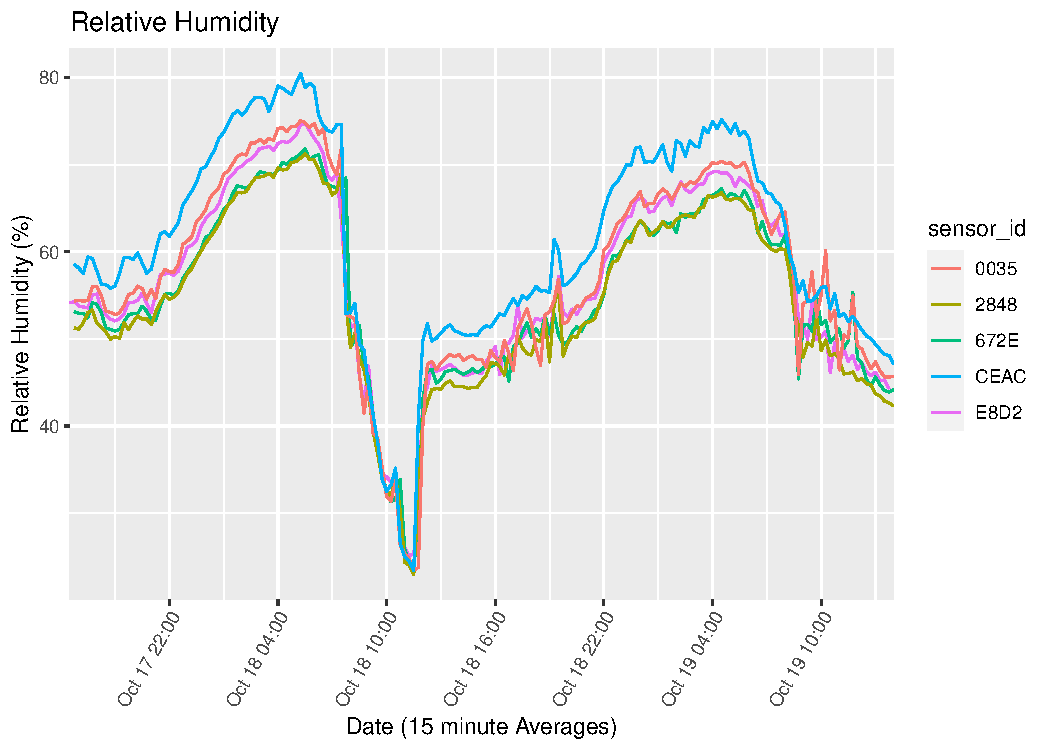
\includegraphics{THP_CEAC_20231102_files/figure-pdf/data_plot_all_rh-1.pdf}

}

\end{figure}

\hypertarget{linear-regression}{%
\section{LINEAR REGRESSION}\label{linear-regression}}

A simple linear regression was performed to compare the CEAC sensor data
to the experimental sensor data. Graphs, output, and equations are shown
below for Temperature and Relative Humidity. Assumptions for a linear
regression were not tested in this exploration.

A linear relationship was found with an R squared of 0.99, and a slope
very near 1.

\begin{Shaded}
\begin{Highlighting}[]
\NormalTok{c }\OtherTok{\textless{}{-}} \FunctionTok{ggplot}\NormalTok{(}\AttributeTok{data =}\NormalTok{ final\_THP\_log\_E8D2, }\FunctionTok{aes}\NormalTok{(}\AttributeTok{x =}\NormalTok{ rh, }\AttributeTok{y =}\NormalTok{ RH\_THREE\_FOOT\_HEIGHT)) }\SpecialCharTok{+}
  \FunctionTok{stat\_poly\_line}\NormalTok{() }\SpecialCharTok{+}
  \FunctionTok{stat\_poly\_eq}\NormalTok{(}\FunctionTok{use\_label}\NormalTok{(}\StringTok{"eq"}\NormalTok{)) }\SpecialCharTok{+}
  \FunctionTok{stat\_poly\_eq}\NormalTok{(}\AttributeTok{label.y =} \FloatTok{0.9}\NormalTok{) }\SpecialCharTok{+}
  \FunctionTok{ggtitle}\NormalTok{(}\StringTok{"RH Linear Regression"}\NormalTok{) }\SpecialCharTok{+}
  \FunctionTok{xlab}\NormalTok{(}\StringTok{"THP RH (\%)"}\NormalTok{) }\SpecialCharTok{+}
  \FunctionTok{ylab}\NormalTok{(}\StringTok{"CEAC RH (\%)"}\NormalTok{) }\SpecialCharTok{+}
  \FunctionTok{geom\_point}\NormalTok{()}


\NormalTok{  t\_model }\OtherTok{=} \FunctionTok{lm}\NormalTok{(RH\_THREE\_FOOT\_HEIGHT }\SpecialCharTok{\textasciitilde{}}\NormalTok{ rh, final\_THP\_log\_E8D2)}
  \FunctionTok{summary}\NormalTok{(t\_model)}
\end{Highlighting}
\end{Shaded}

\begin{verbatim}

Call:
lm(formula = RH_THREE_FOOT_HEIGHT ~ rh, data = final_THP_log_E8D2)

Residuals:
    Min      1Q  Median      3Q     Max 
-7.9605 -0.8117  0.2175  0.9705  8.5323 

Coefficients:
            Estimate Std. Error t value Pr(>|t|)    
(Intercept) -0.77113    0.74434  -1.036    0.302    
rh           1.09234    0.01291  84.624   <2e-16 ***
---
Signif. codes:  0 '***' 0.001 '**' 0.01 '*' 0.05 '.' 0.1 ' ' 1

Residual standard error: 1.888 on 178 degrees of freedom
Multiple R-squared:  0.9757,    Adjusted R-squared:  0.9756 
F-statistic:  7161 on 1 and 178 DF,  p-value: < 2.2e-16
\end{verbatim}

\begin{Shaded}
\begin{Highlighting}[]
\CommentTok{\#get list of residuals}
\NormalTok{res }\OtherTok{\textless{}{-}} \FunctionTok{resid}\NormalTok{(t\_model)}

\CommentTok{\#produce residual vs. fitted plot}
\FunctionTok{plot}\NormalTok{(}\FunctionTok{fitted}\NormalTok{(t\_model), res)}
\CommentTok{\#add a horizontal line at 0}
\FunctionTok{abline}\NormalTok{(}\DecValTok{0}\NormalTok{,}\DecValTok{0}\NormalTok{)}
\end{Highlighting}
\end{Shaded}

\begin{figure}[H]

{\centering 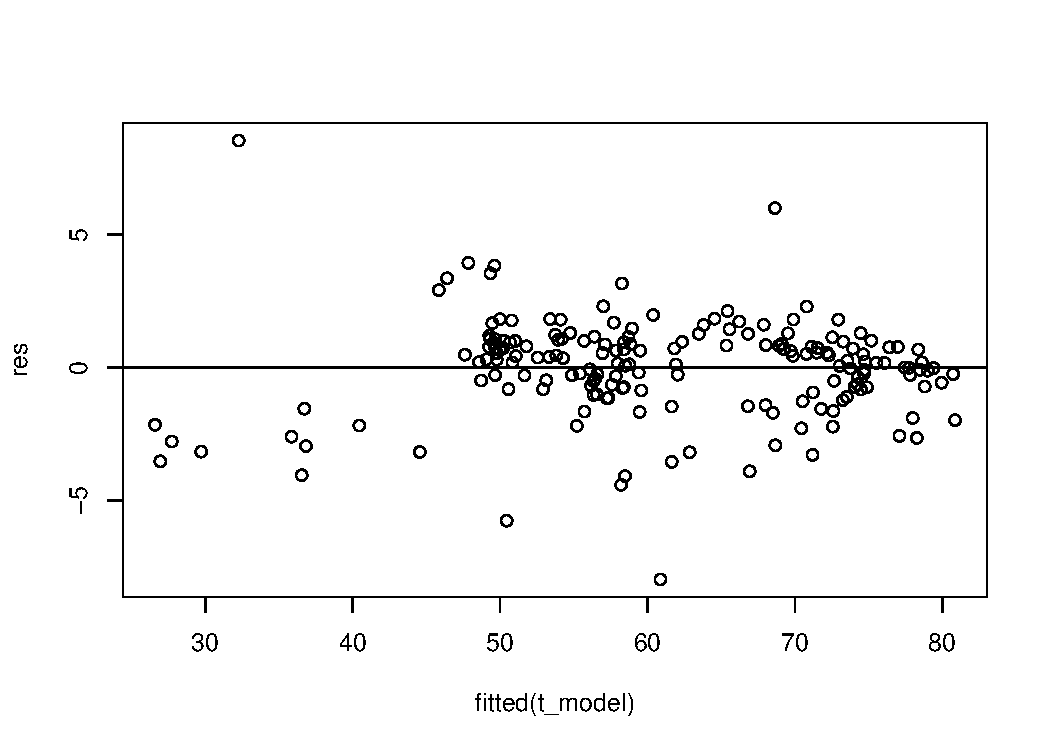
\includegraphics{THP_CEAC_20231102_files/figure-pdf/data_plot_stat_rh-1.pdf}

}

\end{figure}

\begin{Shaded}
\begin{Highlighting}[]
\CommentTok{\#Create density plot of residuals}
\FunctionTok{plot}\NormalTok{(}\FunctionTok{density}\NormalTok{(res))}
\end{Highlighting}
\end{Shaded}

\begin{figure}[H]

{\centering 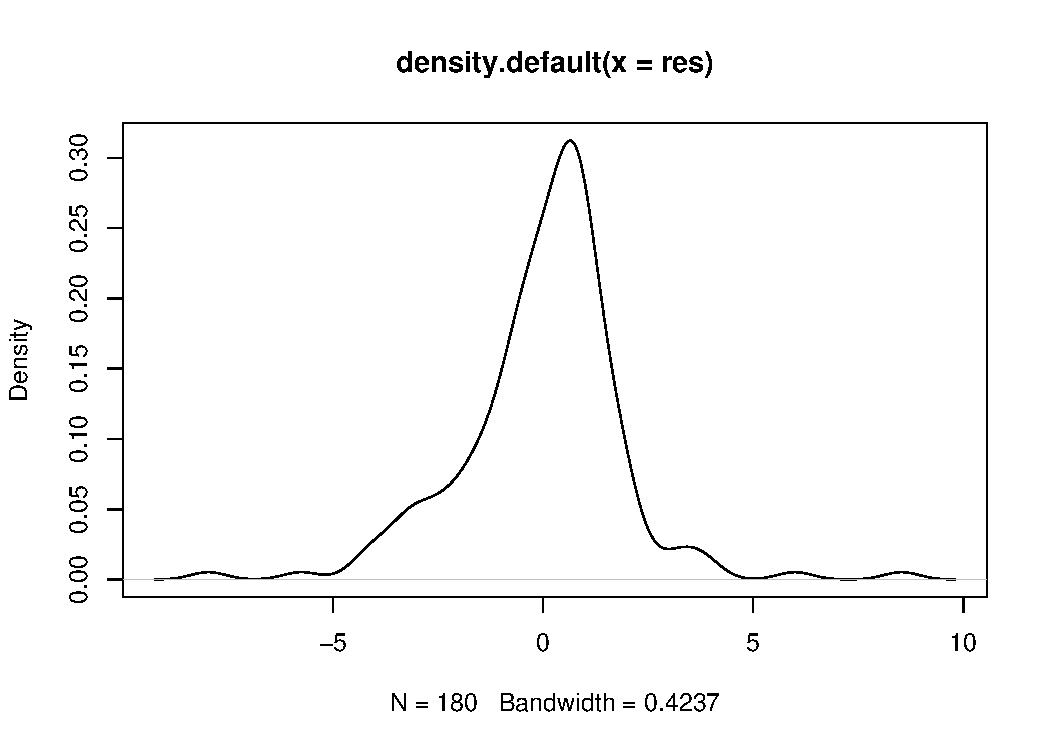
\includegraphics{THP_CEAC_20231102_files/figure-pdf/data_plot_stat_rh-2.pdf}

}

\end{figure}

\begin{Shaded}
\begin{Highlighting}[]
\CommentTok{\#create Q{-}Q plot for residuals}
\FunctionTok{qqnorm}\NormalTok{(res)}
\CommentTok{\#add a straight diagonal line to the plot}
\FunctionTok{qqline}\NormalTok{(res)}
\end{Highlighting}
\end{Shaded}

\begin{figure}[H]

{\centering 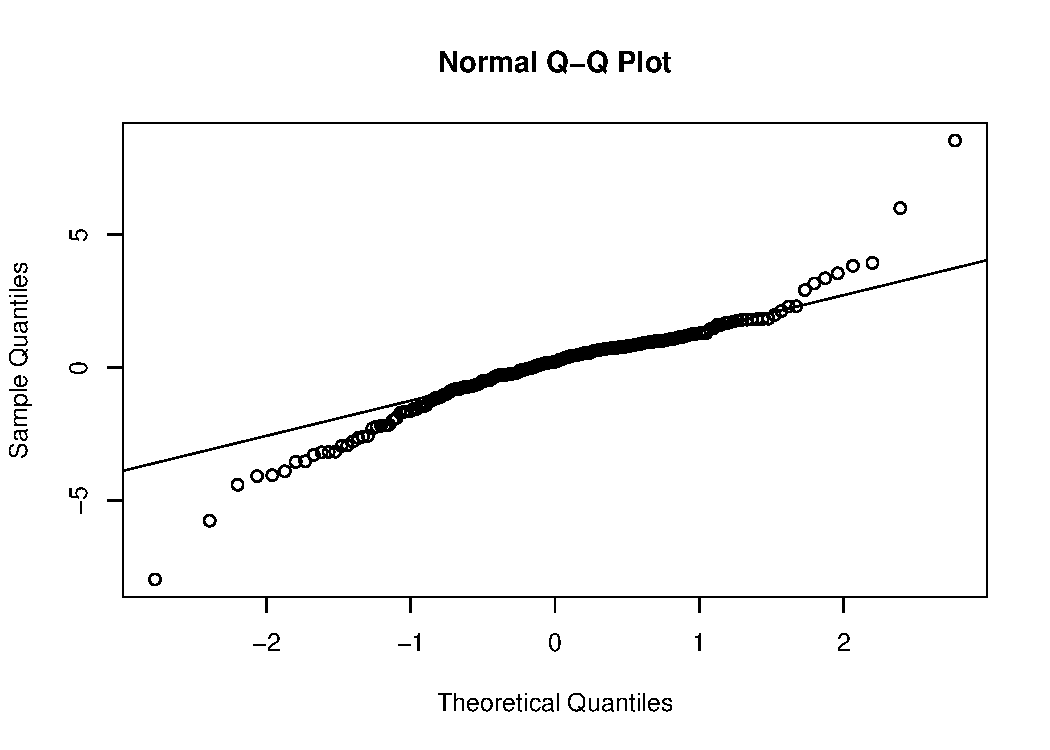
\includegraphics{THP_CEAC_20231102_files/figure-pdf/data_plot_stat_rh-3.pdf}

}

\end{figure}

\begin{Shaded}
\begin{Highlighting}[]
\FunctionTok{library}\NormalTok{(cowplot)}
\end{Highlighting}
\end{Shaded}

\begin{verbatim}
Warning: package 'cowplot' was built under R version 4.2.3
\end{verbatim}

\begin{verbatim}

Attaching package: 'cowplot'
\end{verbatim}

\begin{verbatim}
The following object is masked from 'package:lubridate':

    stamp
\end{verbatim}

\begin{Shaded}
\begin{Highlighting}[]
\FunctionTok{plot\_grid}\NormalTok{(}
\NormalTok{  a,b, c, c,}
  \CommentTok{\# ncol=2,}
  \AttributeTok{labels =} \StringTok{"AUTO"}\NormalTok{,}
  \CommentTok{\# align="hv",}
  \CommentTok{\# rel\_heights = c(2,1),}
  \CommentTok{\# rel\_widths = c(1,2)}
  \AttributeTok{align =} \StringTok{"v"}\NormalTok{, }\AttributeTok{axis =} \StringTok{"b"}\NormalTok{, }\AttributeTok{nrow =} \DecValTok{2}\NormalTok{, }\AttributeTok{rel\_widths =} \FunctionTok{c}\NormalTok{(}\DecValTok{1}\NormalTok{,}\DecValTok{1}\NormalTok{,}\DecValTok{2}\NormalTok{,}\DecValTok{2}\NormalTok{)}
  \CommentTok{\# nrow = 2,}
  \CommentTok{\# rel\_heights = c(1,1,3,3),}
  \CommentTok{\# scale = c(1,1,1.1, 1.1)}
  \CommentTok{\# rel\_widths = c(1, 1,2)}
\NormalTok{  )}
\end{Highlighting}
\end{Shaded}

\begin{figure}[H]

{\centering 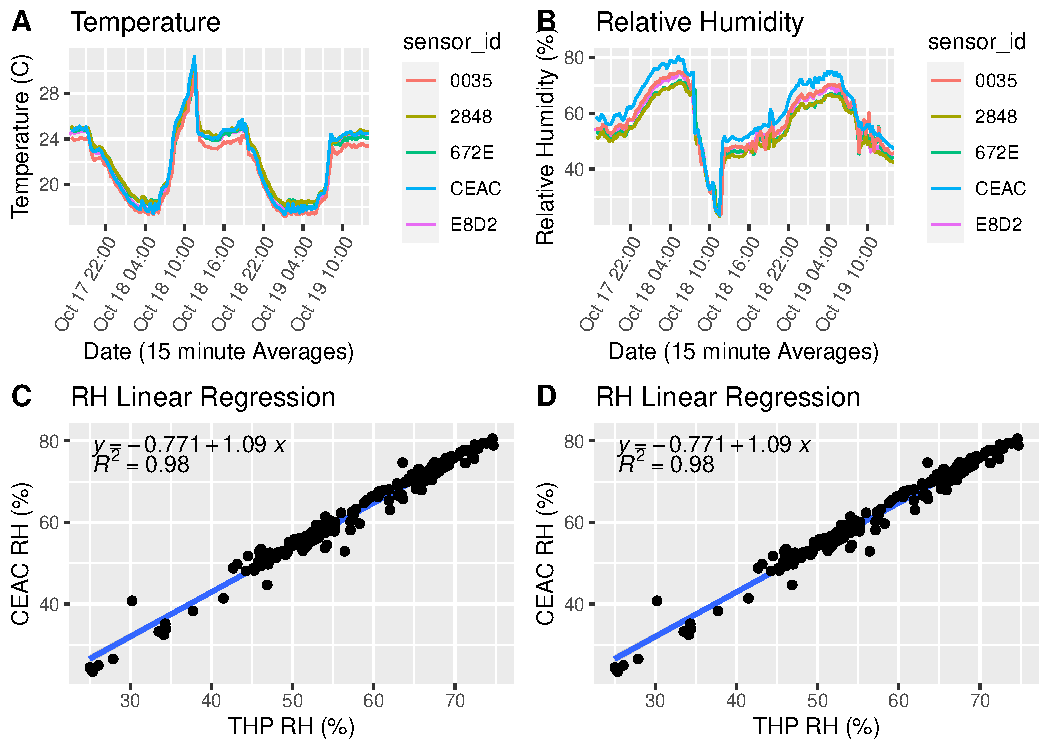
\includegraphics{THP_CEAC_20231102_files/figure-pdf/data_plot_stat_rh-4.pdf}

}

\end{figure}

\begin{Shaded}
\begin{Highlighting}[]
\NormalTok{c}
\end{Highlighting}
\end{Shaded}

\begin{figure}[H]

{\centering 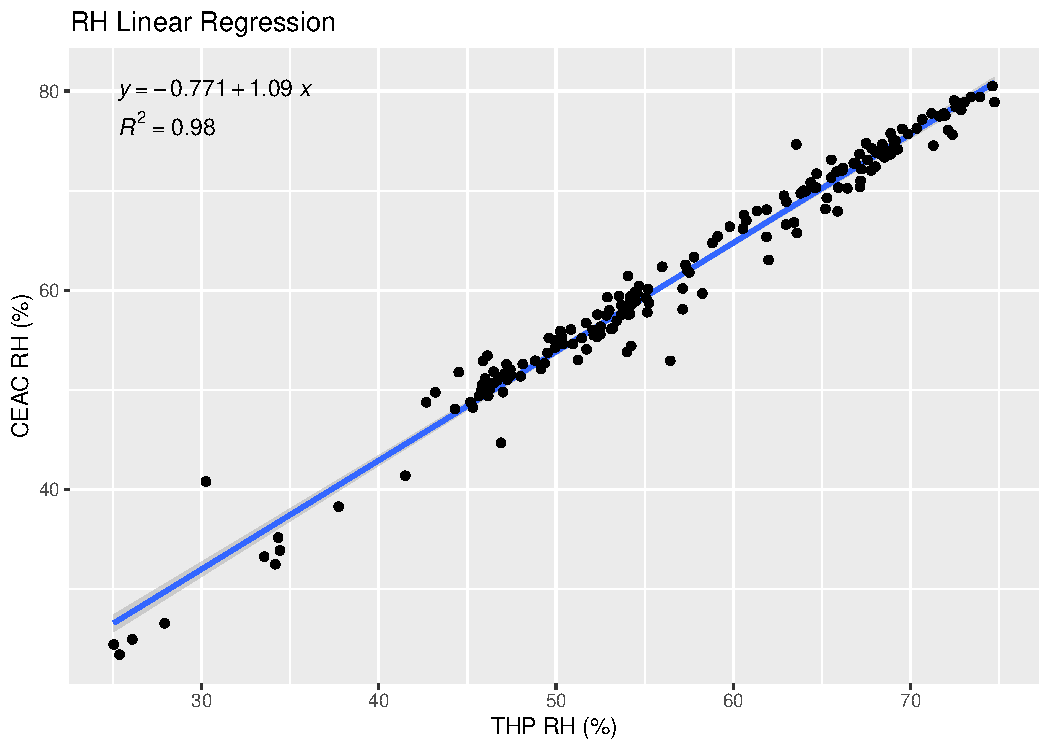
\includegraphics{THP_CEAC_20231102_files/figure-pdf/data_plot_stat_rh-5.pdf}

}

\end{figure}

\hypertarget{discussion}{%
\subsection{DISCUSSION}\label{discussion}}

The test shows a similar response as previous Biosphere 2 sensor tests.
Past comparisons to Biosphere 2 data showed the experimental sensor data
mirrored various Biosphere 2 sensor readings in the tropical rain forest
biome.

The comparison of the experimental sensor with the CEAC sensor shows
similar responses.\\
The statistics show a very good fit for the model. This provides a
calibration equation that can be used during their future use.

\hypertarget{thp-comparison-from-all-4-sensors}{%
\section{THP comparison from all 4
sensors}\label{thp-comparison-from-all-4-sensors}}

\begin{Shaded}
\begin{Highlighting}[]
\CommentTok{\# ggplot(data = finalStats, aes(x = date)) +}
\CommentTok{\#          geom\_line(aes(y = rh, color = "THP Sensor")) +}
\CommentTok{\#          geom\_line(aes(y = RH\_THREE\_FOOT\_HEIGHT, color = "CEAC Sensor")) +}
\CommentTok{\#          ggtitle("RH CEAC vs THP") +}
\CommentTok{\#          xlab("Date (15 minute Averages)") +}
\CommentTok{\#          ylab("Temperature (C)") +}
\CommentTok{\#          \# theme(panel.grid.minor = element\_line(color = 2,}
\CommentTok{\#                                         \# size = 0.25,}
\CommentTok{\#                                         \# linetype = 1)) +}
\CommentTok{\#            scale\_x\_datetime(date\_labels = ("\%b \%d \%H:\%M"),}
\CommentTok{\#           date\_breaks = "6 hours",  expand = expand\_scale(0)) +}
\CommentTok{\#           theme(axis.text.x=element\_text(angle=60, hjust=1))}
\end{Highlighting}
\end{Shaded}




\end{document}
